\section{Product Owner} \label{Roles_SecProductOwner}
\textit{This section will look into our group’s function as the product owners for the semester and how we managed the Backlog.}

%Motivation
As more oversight was required than initially expected, our group accepted the role as product owners for the B\&D subproject group at the end of the 1st sprint. Our tasks were to manage User stories and manage the transition between sprints.

At the same time as the product owners were made, a hierarchy of who the customers were for each subproject. As the product owners of the B\&D subproject, we had the GUI and DB subprojects as our customers.

 \begin{figure}[H]
 	\centering
 	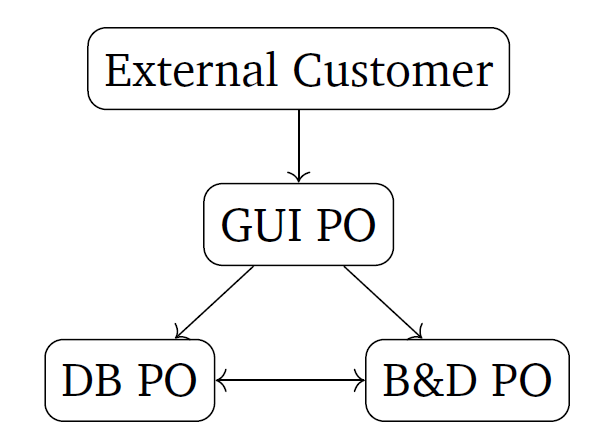
\includegraphics[width=0.6 \textwidth]{pictures/ProductOwnerRelation.png}
 	\caption{Overview of who is customers for who}
 	\label{AppLibependencies}
 \end{figure}
%Sprint Planning
As product owners, we began to chair the sprint planning for our subproject. When sprint planning representatives from the entire project went through every user story in the backlog, and we had the relevant subprojects prioritize the user stories.

After all the user stories were prioritized, the B\&D subproject would by ourselves divide the most important user stories in between us. Given our rather small focus area split between Git, Jenkins, the server, and Google services, most user stories were bound to those roles.

When we were done assigning user stories, each group left to begin work or estimate, depending on their work ethics, after which they could contact us to renegotiate their user stories.

%Sprint - day to day
While the sprint was in operation, there was little to do as product owners. We were expected to keep the backlog updated with new user stories received either from other subprojects or from our own. Other groups were expected to come to us with user stories, that were related to the B\&D subproject..

Otherwise, we held no special distinction in the weekly group meetings or the Scrum meetings held twice a week with the subproject.

%Sprint End
As we began to take over product owner responsibilities, we also began to chair the sprint ends for B\&D. Once all were assembled for the meeting, each group in the subproject would present their work they had done for the sprint. Our Scrum process specified that presentation slides were outlawed for these meetings.

\subsection{Backlog} \label{Roles_SecReleaseBacklog}
As product owners we were in charge of creating and maintaining a backlog for B\&D. In the beginning we used the Redmine tool to maintain a Backlog, however participation across the project groups were low, so the backlog suffered. Shortly after, the product owner groups started using Google Docs to keep track of user stories because Redmine was unwieldy.

At the closure of the second sprint, the product owners started keeping a shared product backlog.

\subsubsection{Release Backlog}
%Introduction + motivation?
In the third sprint we were tasked with making a release backlog for the B\&D subproject as a part of the overall Scrum process and to be able to provide a better overview of what has been made during the semester. At this point, there was no release backlog to speak of, given Redmine's lack of use.

%What is a release backlog
A release backlog is a subset of the product backlog used for Scrum. Where the product backlog is a list of features wanted for the product, the release backlog contains the user stories which have been completed for a given sprint.

With the other product owner groups we put together a shared backlog which contained both the product backlog and the release backlog, to have a common place to find the whole backlog for the next semester’s students. It can be found in Appendix \ref{Appendix_secBacklog}.

%The release backlog
\begin{comment}
\begin{table}
	\centering
	\begin{tabular}{ll}
		\textbf{User Stories} & \textbf{Completed by}\\ \hline \noalign{\vskip 2mm}
		Setting up server & Group 2\\ \hline
		Update to Android 1.0.x & Group 8\\ \hline
		Setting up Git & Group 8\\ \hline
		Google Analytics Setup & Group 5\\ \hline
		Setup of Google Play & Group 5\\ \hline
		Central Documentation & Group 5, 9\\ \hline
		Continuous build and integration & Group 9\\ \hline
		Wiki entry on process & Group 9\\ \hline
	\end{tabular}
	\caption{Release Backlog for sprint 1.}
	\label{Roles_ReleaseBacklogSprint1_table}
\end{table}

\begin{table}
	\centering
	\begin{tabular}{ll}
		\textbf{User Stories} & \textbf{Completed by}\\ \hline \noalign{\vskip 2mm}
		Binaries instead of submodules & Group 5, 8, 9\\ \hline
		Snapshots of database/Backups & Group 2\\ \hline
		SMTP setup & Group 2\\ \hline
		Logging & Group 2\\ \hline
		Gitlab for the server/GOG & Group 2\\ \hline
		Release new APK for Sprint 1 & Group 5\\ \hline
		Auto Upload Beta and Alpha release & Group 9\\ \hline
		Monkey test & Group 9\\ \hline
		Test case installation & Group 9\\ \hline
		Faster build and test & Group 9\\ \hline
		Code coverage & Group 9\\ \hline
		Dependency & Group 9\\ \hline
	\end{tabular}
	\caption{Backlog for sprint 2.}
	\label{Roles_ReleaseBacklogSprint2_table}
\end{table}

\begin{table}
	\centering
	\begin{tabular}{ll}
		\textbf{User Stories} & \textbf{Completed by}\\ \hline \noalign{\vskip 2mm}
		Logging & Group 2\\ \hline
		Symmetric DS & Group 2\\ \hline
		Snapshots of database/Backups & Group 2\\ \hline
		Share the knowledge from Guides & Group 5\\ \hline
		Add a guide on how to do UI test & Group 9\\ \hline
		Make guidelines for Continuous Integration & Group 9\\ \hline
		Specify the Scrum process used & Group 9\\ \hline
		Monkey test & Group 9\\ \hline
		UI test on Jenkins & Group 9\\ \hline
	\end{tabular}
	\caption{Backlog for sprint 3.}
	\label{Roles_ReleaseBacklogSprint3_table}
\end{table}
\end{comment}
